%Auteurs : Nicolas Englebert
\documentclass[british,french,11pt, a4paper, openany]{book}

% Règles de bonne pratiques :
% https://fr.wikibooks.org/wiki/LaTeX/Gestion_des_gros_documents

%%%%%%%%%%%%%%%%
%%% Packages %%%
%%%%%%%%%%%%%%%%

%%% Compatibilité %%%
\begingroup\expandafter\expandafter\expandafter\endgroup
\expandafter\ifx\csname IncludeInRelease\endcsname\relax
\usepackage{fixltx2e}
\fi 					% Si version LaTeX < 2015, inclut un fix.

%%% Général %%%
\usepackage[utf8]{inputenc}
\usepackage{babel}
\usepackage{lmodern}
\usepackage[T1]{fontenc}
\addto\extrasfrench{\sisetup{locale = FR,detect-all}} % Switch siunitx en fonction de la langue babel :)
\addto\extrasbritish{\sisetup{locale = UK,detect-all}}
\usepackage{courier}
\usepackage{graphicx}
%\usepackage{cancel}

%%% Tableau %%%
%\usepackage{tabularx} %Permet d'auto dimensionner les tableaux



%%% Bibliographie %%%
%\usepackage[style=alphabetic,backend=biber]{biblatex}
\usepackage[autostyle]{csquotes}
%\DeclareNameAlias{sortname}{last-first}
%\DeclareFieldFormat{url}{\space\url{#1}}
%\DeclareNameAlias{labelname}{last-first}
%\addbibresource{sample.bib}


%%% Graphiques %%%
%\usepackage{tikz}
%\usepackage{pgfplots}
%\usepackage{circuitikz}

%%% Mise en page %%%
\usepackage{mathtools}
\usepackage{amssymb}
\usepackage{bbm}
\usepackage{amsthm}
%\usepackage[tt]{titlepic}% Centre le titre
%\usepackage{fancyhdr}   % Permet de modifier l'entête & footer
\usepackage{caption}     % Permet d'ajouter des légendes en images sans les mettre en float + dans la marge + ref vers le haut de l'envirronement
\usepackage{wrapfig}
\usepackage{fullpage}
%\usepackage{multicol}   % pour les liste sur plusieurs colonnes
%\usepackage{subfigure}  % alligne deux images cote a cote
\usepackage{float}      %permet de mettre du texte entre les figures grace a [H]. Génial! 
\usepackage{eso-pic}    % Fond d'écran page de garde
\usepackage{adjustbox}  % Empêche les box de sortir de la page


%%% Math %%%
%\usepackage{delarray} % Belles matrices
\usepackage{siunitx}


%%% Codes %%%
%\usepackage{listings}
%\usepackage[final]{pdfpages} %% Inclusion fichier pdf

%% Reference
\usepackage{hyperref}
%\renewcommand*{\figureautorefname}{fig.}
%\def\appendixautorefname{annexe}
%\def\tableautorefname{tab.}
%\renewcommand*{\chapterautorefname}{ch.}
%\newcommand{\subfigureautorefname}{\figureautorefname}



%%%%%%%%%%%%%%%%%
%%% Commandes %%%
%%%%%%%%%%%%%%%%%

%%% Physique %%%
\newcommand{\cst}{\text{cst}}
\newcommand{\D}{\partial}
\newcommand{\E}{\vec E}
\newcommand{\B}{\vec B}
\newcommand{\F}{\vec F}
\newcommand{\modu}[1]{|$#1$|}

%%% Math %%%
\newcommand{\oiint}{\int\!\!\!\!\!\!\! \:\!\subset\!\!\supset\!\!\!\!\!\!\!\int}
\newcommand{\rot}{\operatorname{\vec{rot}}}
\newcommand{\divv}{\operatorname{div}}
\newcommand{\phas}[1]{\underline{#1}}
\newcommand{\RE}{\text{Re}}
\newcommand{\ft}{\overset{\mathcal{F}}{\longleftrightarrow}}
\newcommand{\lt}{\overset{\mathcal{L}}{\longleftrightarrow}}
\newcommand{\DS}{\displaystyle}
\newcommand{\Tr}{\operatorname{Tr}}



%% Box
\shorthandon{:}
\newcommand{\theor}[1]{\adjustbox{minipage=\linewidth-2\fboxsep-2\fboxrule,fbox}{\textsc{\iflanguage{british}{Theorem}{Théorème}: }#1}}
\newcommand{\defi}[1]{\adjustbox{minipage=\linewidth-2\fboxsep-2\fboxrule,fbox}{\textsc{\iflanguage{british}{Definition}{Définition}: }#1}}
\newcommand{\lemme}[1]{\adjustbox{minipage=\linewidth-2\fboxsep-2\fboxrule,fbox}{\textsc{\iflanguage{british}{Lemma}{Lemme}: }#1}}
\newcommand{\prop}[1]{\adjustbox{minipage=\linewidth-2\fboxsep-2\fboxrule,fbox}{\textsc{\iflanguage{british}{Property}{Propriété}}\\ #1}}
\newcommand{\proposition}[1]{\adjustbox{minipage=\linewidth-2\fboxsep-2\fboxrule,fbox}{\textsc{Proposition}\\#1}}
\newcommand{\cadre}[1]{\adjustbox{minipage=\linewidth-2\fboxsep-2\fboxrule,fbox}{#1}}
\newcommand{\retenir}[1]{\adjustbox{minipage=\linewidth-2\fboxsep-2\fboxrule,fbox}{\textbf{\textit{\textsc{\iflanguage{british}{To remember}{À retenir}}: }}#1}}

\newcommand{\corollaire}[1]{\bigbreak\begin{tabular}{||c}
	\begin{minipage}{\textwidth}
		\textsc{\iflanguage{british}{Corollary}{Corollaire}: } \textit{#1}
	\end{minipage}
	\end{tabular}}
\newcommand{\exemple}[1]{\bigbreak\begin{tabular}{|c}
	\begin{minipage}{\textwidth}
		\textsc{\iflanguage{british}{Example}{Exemple}: } #1
	\end{minipage}%
	\end{tabular}}%
\shorthandoff{:}
    

%\pagestyle{headings} % Titre du ch et numéro page dans l'entete
%\renewcommand{\proofname}{Démonstration}
%\addto\captionsfrench{\def\tablename{Tableau}}


%%% Background %%%
\newcommand\BackgroundPic{%
	\put(0,0){%
		\parbox[b][\paperheight]{\paperwidth}{%
			\vfill
			\centering
			\includegraphics[width=\paperwidth,height=\paperheight,%
			keepaspectratio]{../../Builder/ulb.jpg}%
			\vfill
}}}

%%% Annexes Cedu %%%
%\usepackage{calrsfs}
%\DeclareMathAlphabet{\pazocal}{OMS}{zplm}{m}{n}
\usepackage{fourier-orns}

\setlength{\parindent}{0pt} 

%%% Attributs %%%
\newcommand*{\NomduCours}[2]{\def\cours{#1}\def\memo{#2}}
\newcommand*{\annee}[2]{\def\adebut{#1}\def\afin{#2}}

\newcounter{auteurcnt}
\newcommand\addauteur[2]{%
	\stepcounter{auteurcnt}%
	\csdef{auteur\theauteurcnt}{\mbox{#1~\textsc{#2}}}}
\newcommand\getauteur[1]{%
	\csuse{auteur#1}}

\newcounter{illustrateurcnt}
\newcommand\addillustrateur[2]{%
	\stepcounter{illustrateurcnt}%
	\csdef{illustrateur\theillustrateurcnt}{\mbox{#1~\textsc{#2}}}}
\newcommand\getillustrateur[1]{%
	\csuse{illustrateur#1}}

\newcounter{rappeltheocnt}
\newcommand\addrappeltheo[2]{%
	\stepcounter{rappeltheocnt}%
	\csdef{rappeltheo\therappeltheocnt}{\mbox{#1~\textsc{#2}}}}
\newcommand\getrappeltheo[1]{%
	\csuse{rappeltheo#1}}

\newcounter{professeurcnt}
\newcommand\addprofesseur[2]{%
	\stepcounter{professeurcnt}%
	\csdef{professeur\theprofesseurcnt}{\mbox{#1~\textsc{#2}}}}
\newcommand\getprofesseur[1]{%
	\csuse{professeur#1}}

\newcounter{iter}

%Typique Phys
\usepackage{physics}
\usepackage{multicol}

% Attributs
\NomduCours{Physique atomique}{PHYS-H-405}
\addauteur{Nicolas}{Englebert}
\addprofesseur{Michel}{Godefroid}
\annee{2016}{2017}


% Document
\begin{document}
\def\equationautorefname~#1\null{%
	(#1)\null
}
\newcommand{\notes}[1]{\bigbreak\begin{tabular}{|c}
		\begin{minipage}{\textwidth}
			#1
		\end{minipage}%
\end{tabular}}%
%%%%%%%%%%%%%%%%%
% Préliminaires %
%%%%%%%%%%%%%%%%%
\frontmatter
\AddToShipoutPicture*{\BackgroundPic}

\begin{titlepage}
	\begin{center}	
			
		\newcommand{\HRule}{\rule{\linewidth}{0.5mm}}   			            %Titre en gros
		\includegraphics[width=0.55\textwidth]{../../Builder/titlepage/logo.pdf}~\\[1cm]				%Logo
			
			\textsc{\LARGE Université Libre de Bruxelles}\\[1.5cm]
			\textsc{\Large \iflanguage{british}{Summary}{Synthèse}}\\[0.5cm]
			
			\HRule \\[0.4cm]
			{ \huge \bfseries \cours \ \\\memo \\[0.4cm] }
			
			
			\HRule \\[1.5cm]
			\begin{minipage}[t]{0.6\textwidth}
				\begin{flushleft}%\large
					\emph{\iflanguage{british}{Author}{Auteur}\ifnum\theauteurcnt>1 s\fi:}\\
					\whileboolexpr
					{ test {\ifnumcomp{\value{iter}}{<}{\theauteurcnt}} }%
					{\stepcounter{iter}\getauteur{\theiter}\\}
					\setcounter{iter}{0}%
					\ifnum\theillustrateurcnt>0%
					\ \\
					\emph{Illustrations:}\\
					\whileboolexpr
					{ test {\ifnumcomp{\value{iter}}{<}{\theillustrateurcnt}} }%
					{\stepcounter{iter}\getillustrateur{\theiter}\\}%
					\setcounter{iter}{0}%
					\fi%
					\ifnum\therappeltheocnt>0%
					\ \\
					\emph{\iflanguage{british}{Reminders}{Rappels théoriques}:}\\
					\whileboolexpr
					{ test {\ifnumcomp{\value{iter}}{<}{\therappeltheocnt}} }%
					{\stepcounter{iter}\getrappeltheo{\theiter}\\}%
					\setcounter{iter}{0}%
					\fi%
				\end{flushleft}
			\end{minipage}%
			\begin{minipage}[t]{0.25\textwidth}
				%\begin{flushright}
				%\large
				\emph{\iflanguage{british}{Professor}{Professeur}\ifnum\theprofesseurcnt>1 s\fi:}
				\whileboolexpr
				{ test {\ifnumcomp{\value{iter}}{<}{\theprofesseurcnt}} }%
				{\\ \stepcounter{iter}\getprofesseur{\theiter}}%
				\setcounter{iter}{0}%
				%\end{flushright}
			\end{minipage}
			
			\vfill
			
			% Bottom of the page
			{\large \iflanguage{british}{Year}{Année} \adebut~-~\afin}
			
		\end{center}
	\end{titlepage}

\ \\[2cm]
{\Huge \bfseries Appel à contribution}\\[5mm]
\subsection*{Synthèse Open Source}
\begin{wrapfigure}[5]{l}{4.5cm}
	\includegraphics[scale=0.5]{../../Builder/git.png}
\end{wrapfigure}
Ce document est grandement inspiré de l’excellent cours donné 
par \ifnum\theprofesseurcnt=1 \getprofesseur{1} \else\whileboolexpr
{ test {\ifnumcomp{\value{iter}}{<}{\theprofesseurcnt-2}} }%
{\stepcounter{iter}\getprofesseur{\theiter}, }%
\stepcounter{iter}\getprofesseur{\theiter} et \stepcounter{iter}\getprofesseur{\theiter} \fi%
 à l’EPB (École Polytechnique de Bruxelles), faculté de l’ULB (Université 
Libre de Bruxelles). Il est écrit par les auteurs susnommés avec l’aide de tous les autres étudiants 
et votre aide est la bienvenue ! En effet, il y a toujours moyen de l’améliorer surtout que si le 
cours change, la synthèse doit être changée en conséquence. On peut retrouver le code source à l’adresse 
suivante
\begin{center}
	\url{https://github.com/nenglebert/Syntheses}
\end{center}\bigskip
Pour contribuer à cette synthèse, il vous suffira de créer un compte sur \textit{Github.com}. De
légères modifications (petites coquilles, orthographe, ...) peuvent directement être faites sur le
site ! Vous avez vu une petite faute ? Si oui, la corriger de cette façon ne prendra que quelques 
secondes, une bonne raison de le faire ! \bigskip

Pour de plus longues modifications, il est intéressant de disposer des fichiers : il vous 
faudra pour cela installer \LaTeX, mais aussi \textit{git}. Si cela pose problème, nous sommes 
évidemment ouverts à des contributeurs envoyant leur changement par mail ou n’importe quel autre 
moyen.\bigskip

Le lien donné ci-dessus contient aussi un \texttt{README} contenant de plus amples informations, 
vous êtes invités à le lire si vous voulez faire avancer ce projet ! 

\subsection*{Licence Creative Commons}
\begin{wrapfigure}[3]{r}{2.8cm}
	\vspace{-5mm}
	\includegraphics[scale=0.17]{../../Builder/CC}
\end{wrapfigure}
Le contenu de ce document est sous la licence Creative Commons : \textit{Attribution-NonCommercial-ShareAlike 
4.0 International (CC BY-NC-SA 4.0)}. Celle-ci vous autorise à l'exploiter pleinement, compte-
tenu de trois choses :
\begin{enumerate}
	\item \textit{Attribution} ; si vous utilisez/modifiez ce document vous devez signaler le(s) nom(s)
	      de(s) auteur(s).
	\item \textit{Non Commercial} ; interdiction de tirer un profit commercial de l’œuvre sans 
	      autorisation de l'auteur 
	\item \textit{Share alike} ;  partage de l’œuvre, avec obligation de rediffuser selon la même 
	      licence ou une licence similaire
\end{enumerate}
Si vous voulez en savoir plus sur cette licence :
\begin{center}
	\url{http://creativecommons.org/licenses/by-nc-sa/4.0/}
\end{center}

\begin{flushright}
	\textbf{Merci ! }
\end{flushright}
\tableofcontents
%Si abstract, \input ici

%%%%%%%%%%%%%%%%%%%%%
% Contenu principal %
%%%%%%%%%%%%%%%%%%%%%
\mainmatter
\chapter{Interaction des particules chargées avec la matière : considérations de base}
\section{Introduction}
Il existe trois types de rayonnements ionisants (\textit{ionizing radiations})
\begin{enumerate}
\item Les particules chargées
\begin{itemize}
\item Électron, positron, ions, \dots
\end{itemize}
\item Les photons (particules neutres sans masses)
	\begin{itemize}
	\item Les $\gamma$ (origine \textbf{nucléaire})
	\item Les $X$ (origine atomique)
	\end{itemize}
\item Neutrons (particules neutres)
\end{enumerate}
Notons que ce qui fait vraiment la différence entre un $\gamma$ et un $X$ est le mode 
d'émission et non pas l'énergie (conséquence).\\

Pour chacun de ces types de rayonnement, il existe un mécanisme d'interaction particulier
avec la matière\footnote{\textit{Assemblage d'atomes isolés sans interaction entre-eux : 
gaz d'atome}. Il s'agit de la définition de ce cours, qui évoluera au fil des chapitres}. 
\begin{itemize}
\item[$\bullet$] Les particules chargées interagissent par interactions coulombienne 
(noyaux et électrons), les collisions sont donc fréquentes et on peut considérer que 
l'énergie est perdue de façon (quasi-)continue. La particule s'arrête ainsi à distance 
finie dans la matière de sorte à ce qu'on puisse définir un "parcours" (\textit{range}) 
de celle ci  : de tels rayonnements sont \textit{directement} ionisants
\item[$\bullet$] Les particules neutres (pas d'interaction coulombienne) ont une 
probabilité de traverser la matière sans interactions, il n'est donc pas possible de 
définir un range. Elles peuvent par contre déposées de l'énergie à des particules 
chargées qui vont causés une ionisation : de tels rayonnements sont \textit{indirectement} 
ionisants
\end{itemize}
Les interactions d'un rayonnement avec la matière peut modifier l'état du rayonnement 
(absorbé, dévié, \dots) et aussi l'état de la matière (excités, ionisés,\dots).

\newpage
\subsection{Interaction des particules chargées avec la matière}
	\begin{wrapfigure}[7]{l}{6cm}
	\vspace{2mm}
	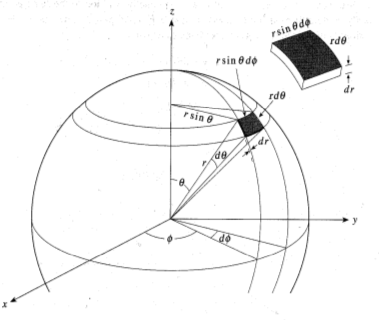
\includegraphics[scale=0.4]{ch1/image1.png}
	\captionof{figure}{Trajectoire d'une particule chargée}
	\end{wrapfigure}
Comme annoncé ci-dessus, les particules chargées subissent des collisions 
coulombiennes\footnote{Les réactions nucléaires sont laissées de côté.} avec :
\begin{description}
\item[Les noyaux (rare)] : cause une importante perte d'énergie et une grande déviation
angulaire
\item[Les électrons (fréquent)] : cause des excitations/ionisations se traduisant par des
faibles pertes d'énergie et déviations angulaires
\end{description}\ \\

	\begin{wrapfigure}[7]{r}{6cm}
	\vspace{-9mm}
	\includegraphics[scale=0.4]{ch1/image2.png}
	\captionof{figure}{ }
	\end{wrapfigure}
Chaque collision cause alors une perte d'énergie $T_j$, causés par un grand nombre de 
projectiles $N$ qui suivent $N$ histoires propres : le nombre de collision étant très 
important, les fluctuations sont faibles et il devient possible de définir des quantités
moyennes.\\

Pour introduire ces valeurs moyennes, il faut avant tout introduire la notion de 
\textbf{section efficace}.\ \\

\cadre{La \textbf{section efficace} est l'aire fictive que doit avoir une particule incidente
pour reproduire la probabilité de collision observée avec une particule cible.}\ \\

	\begin{wrapfigure}[7]{l}{6cm}
	\vspace{-5mm}
	\includegraphics[scale=0.5]{ch1/image3.png}
	\captionof{figure}{ }
	\end{wrapfigure}
Il existe plusieurs sortes de section efficace. Pour s'en rendre compte, définissons ce
qu'est une collision. Il s'agit de \textit{l'interaction entre une particule incidente et une particule cible qui implique un effet spécifique mesurable}. Ainsi, la section efficace ne 
dépend pas que des particules incidentes/cibles et de leur vitesse \textbf{mais aussi} de l'effet
physique !\\
\ \\

Sur le grand nombre d'interaction existant, on peut s'intéresser à une perte d'énergie 
(section efficace différentielle en énergie $d\sigma/dE$) ou à une émission dans une 
direction donnée ((section efficace différentielle en énergie $d\sigma/d\Omega$).\\

	\begin{wrapfigure}[7]{r}{5cm}
	\vspace{-9mm}
	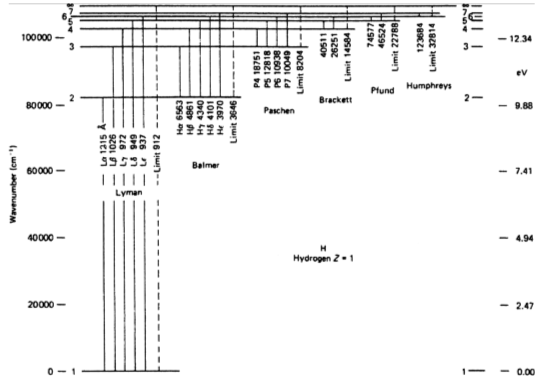
\includegraphics[scale=0.5]{ch1/image4.png}
	\captionof{figure}{ }
	\end{wrapfigure}
Quel est le rapport avec les valeurs moyennes annoncées ci-dessus ? Il n'est pas possible 
de déterminer expérimentalement les sections efficaces microscopiques en bombardant un 
atome avec une seule particule, il va falloir travailler avec des informations 
\textbf{statistiques} venant d'un bombardement (faisceau) sur la matière (milieu). Nous 
ferons l'hypothèse que les projectiles du faisceau n'interagissent pas entre-eux.\newpage

	\begin{wrapfigure}[9]{r}{4cm}
%	\vspace{-9mm}
	\includegraphics[scale=0.35]{ch1/image5.png}
	\captionof{figure}{ }
	\end{wrapfigure}
La section efficace sera ainsi définie par une probabilité. Soit un faisceau de particule
(densité de courant $J$), un milieu cible (aire $S$ plus petites que l'aire du faisceau)
et processus d'interaction $A$ (caractérisé par $\sigma_A$). Le nombre d'interaction $A$ 
induits par le faisceau par unité de temps $n_A$ s'écrit
\begin{equation}
n_A=JS\times\frac{\sigma_A}{S}=J\sigma_A
\end{equation}\ \\
Considérons un volume $V=S.x$ et une densité de particule cible $N$ 
\begin{equation}
n_A=N\times Sx\times J\sigma_A=JS\times Nx\sigma_A\quad\Rightarrow\quad P_A=Nx\sigma_A
 {\mbox{~~~~pour~~~~}}Nx\sigma_A\ll 1
\end{equation}
où $P_A$ est la probabilité pour un projectile de subir un processus $A$.\\

Dans le cas où $N.x.\sigma_A$ n'est pas petit, on peut observer une collision et, s'il 
n'y a pas d'absorption, la particule peut en subir une nouvelle : on parle de \textbf{
collisions multiples}. Soit $P_n$ la probabilité d'initier $n$ événements $A$. Cette 
situation est équivalente à considérer $n$ particules cibles dans un cylindre de volume 
$v=x.\sigma_A$ associé à une trajectoire. Ce problème est un classique de la théorie 
cinétique des gaz, on peut montrer que $P_n$ quit une distribution de Poisson
\begin{equation}
P_n=\frac{(Nv)^n}{n!}e^{-Nv}
\end{equation}
La valeur moyenne se définit alors comme
\begin{equation}
\langle n \rangle=Nv=Nx\sigma_A
\end{equation}
On en tire la \textsc{Loi de Lambert \& Beer} gouvernant les phénomènes d'absorption
\begin{equation}
P_0=e^{-Nx\sigma_A}
\end{equation}
Il s'agit de la probabilité de ne pas se faire absorbé. Si $Nx\sigma_A\ll 1$, on peut 
utiliser l'approximation suivante
\begin{equation}
P_n\simeq\left\{
\begin{aligned}
   &1-Nx\sigma_A& {\mbox{~~~~pour~~~~}} n=0\\
   &Nx\sigma_A& {\mbox{~~~~pour~~~~}} n=1\\
   &0&{\mbox{~~~~pour~~~~}} n\ge 2
\end{aligned} 
\right.
\end{equation}
Cette distribution nous permet de définir aisément la distance moyenne entre deux 
processus de type $A$, soit le \textbf{libre parcours moyen $\lambda_A$}
\begin{equation}
\lambda_A=\frac{1}{N\sigma_A}
\end{equation}
Ceci se généralise pour les processus multiples
\begin{equation}
\sigma_{total}=\sigma_A+\sigma_B+\sigma_C+\dots,\qquad \frac{1}{\lambda_{total}}=\frac{1}{\lambda_{A}}+\frac{1}{\lambda_{B}}+\frac{1}{\lambda_{C}}+\dots
\end{equation}


\subsubsection{Pouvoir d'arrêt}
Les pertes en énergies sont caractérisée par le \textbf{pouvoir d'arrêt} (\textit{stopping power}) : il s'agit de la grandeur la plus importante pour une particule chargée. Il s'agit - pour une 
particule chargée d'énergie cinétique $E$ dans un matériau - de la perte d'énergie moyenne
($\Delta E$) par unité de longueur subie par la particule le long de sa trajectoire ($\Delta x$)
\begin{equation}
\dfrac{\Delta E}{\Delta x}\qquad [J.M^{-1}] = [eV.m^{-1}]
\end{equation}
Afin de l'exprimer mathématiquement, considérons une cible de petite épaisseur (par rapport 
à la profondeur de pénétration) $\Delta x$ et un projectile d'énergie $E$. En considérant des 
pertes d'énergies discrète $T_j \ll E$ :
\begin{equation}
\Delta E = \sum_j n_jT_j
\end{equation}
L'énergie moyenne se calcule donc
\begin{equation}
\langle \Delta E \rangle= \sum_j \langle n_j \rangle T_j
\end{equation}
où $\langle n_j\rangle=N\Delta x\sigma_j$. Nous avons alors
\begin{equation}
\langle \Delta E \rangle = N \Delta x \sum_j T_j \sigma_j
\end{equation}
En définissant la \textbf{section efficace d'arrêt} $S$
\begin{equation}
S = \sum T_j\sigma_j
\end{equation}
On définit le \textbf{pouvoir d'arrêt}\ \\

\cadre{\begin{equation}
\frac{\langle \Delta E \rangle}{\Delta x}= NS=N\sum_j T_j \sigma_j
\end{equation}}\ \\

Le pouvoir d'arrêt est donc une propriété \textit{macroscopique} tandis que la section 
efficace d'arrêt est une propriété \textit{microscopique}.

\subsubsection{Paramètres de straggling}
Tant que nous sommes dans les statistiques, calculons les écarts quadratiques moyens des
fluctuations en énergie
\begin{equation}
\Omega^2=\overline{(\Delta E-\langle \Delta E \rangle)^2}
\end{equation}
En considérant $\Delta E-\langle \Delta E \rangle= \sum_j (n_j-\langle n_j \rangle) T_j$, 
on obtient
\begin{equation}
\overline{(\Delta E-\langle \Delta E \rangle)^2}= \sum_{j ,l}\overline{(n_j-\langle n_j \rangle) (n_l-\langle n_l \rangle)}T_jT_l
\end{equation}
Deux cas sont possibles
\begin{enumerate}
\item $j=l$; on peut utiliser les propriétés de la distribution de Poisson
\begin{equation}
\overline{(n_j-\langle n_j \rangle)^2}=\langle n_j \rangle=N\Delta x \sigma_j
\end{equation}
\item $j\neq m$; on transforme la moyenne du produit en produit des moyennes 
(ceci suggère l'indépendance statistiques des différents types de collisions)
\begin{equation}
\overline{(n_j-\langle n_j \rangle) (n_l-\langle n_l \rangle)}=\overline{(n_j-\langle n_j \rangle)}\times\overline{(n_l-\langle n_l \rangle)}
\end{equation}
Or, comme $\overline{n_j-\langle n_j \rangle}=0$, les termes avec $j\neq l$ sont nuls
\end{enumerate}
On obtient donc
\begin{equation}
\Omega^2=\sum_j\langle n_j \rangle T_j^2=N\Delta x\sum_jT_j^2\sigma_j=N\Delta xW
\end{equation}
où $W$ est le \textbf{paramètre de straggling} qui \textit{caractérise les fluctuations en 
énergie} et est défini comme\footnote{Paramètre microscopique.}\ \\

\cadre{\begin{equation}
W=\sum_j T_j^2 \sigma_j
\end{equation}}\ \\

\subsubsection{Notation intégrale et cible épaisse}
Comme annoncé, le grand nombre de collision implique une perte d'énergie quasi-continue (et 
donc un spectre continu)
\begin{equation}
\sigma_j \rightarrow \frac{d\sigma}{dT}\Delta T_j
\end{equation}
Si $\Delta T_j$ est suffisamment petit, les sommes deviennent des intégrales\ \\

\cadre{\begin{equation}
S = \int T\ d\sigma,\qquad\qquad\qquad W = \int T^2 d\sigma
\end{equation}
où $d\sigma =  \frac{d\sigma}{dT}dT$.}\ \\

Nous avions jusqu'ici considéré $\Delta x$ petit impliquant $E$ constant, mais en général $S$
et $W$ dépendent de $E$. En considérant que les fluctuations des pertes d'énergies sont 
négligeables, l'énergie $E$ est bien définie en fonction de la profondeur de pénétration 
$x$\footnote{$E\to E(x)$}. On fait alors l'\textit{approximation du ralentissement continu}
(\textit{Continuous Slowing Down Approximation} - CSDA)\ \\

\cadre{\begin{equation}
\dfrac{dE}{dx} = -NS(E)
\end{equation}
où le signe négatif tient compte de la diminution d'énergie du projectile.}\ \\

Le parcours (\textit{range}) $R$ d'une particule chargée d'énergie $E$ dans un milieu est 
la valeur moyenne $\langle l \rangle$ de la longueur $l$ de sa trajectoire suivie 
jusqu'à son arrêt (sans tenir compte du mouvement thermique). En CSDA, on trouve comme 
profondeur de pénétration
\begin{equation}
x=\int^{E}_{E(x)}\frac{dE'}{NS(E')}
\end{equation}
Le \textit{range} en CSDA est donné pour $x=l$ avec $E(l)=0$
\begin{equation}
R_{CSDA}=\int^{E}_{0}\frac{dE'}{NS(E')}
\end{equation}
Rappelons que cette expression valable pour un straggling en énergie négligeable, à cause 
de notre première hypothèse.


\subsubsection{Modèle classique du pouvoir d'arrêt}
Il s'agit d'un modèle classique non-relativiste établi en 1913 par Niels \textsc{Bohr} qui
est incroyablement correct pour une certaine plage d'énergie.\\

	\begin{wrapfigure}[7]{l}{7cm}
	\vspace{-8mm}
	\includegraphics[scale=0.55]{ch1/image6.png}
	\captionof{figure}{ }
	\label{fig:1.6}
	\end{wrapfigure}
Soit un projectile de charge $e_1$, de masse $m_1$, de vitesse $v$ et une particule cible
($m_2,e_2$) initialement \textbf{au repos}. Cette condition initiale implique un 
\textit{scattering de Coulomb} avec un paramètre d'impact $p$\footnote{Pour rappel, il 
s'agit de la distance entre la trajectoire initiale de 1 et 2.} supposé \textit{pas trop 
petit} (\textit{soft collision}).\\

	\begin{wrapfigure}[9]{r}{6cm}
	\vspace{-8mm}
	\includegraphics[scale=0.55]{ch1/image7.png}
	\captionof{figure}{ }
	\end{wrapfigure}
Supposons que la particule cible reçoit une quantité de mouvement faible tel qu'elle peut 
être considérée au repos durant l'interaction : on note le transfert de la quantité de
mouvement (unités CGS)
\begin{equation}
\overrightarrow{\Delta P}=\int_{-\infty}^{+\infty} dt \overrightarrow{F}(t)
\end{equation}
où $\DS F(t)=\frac{e_1e_2}{p^2+(vt)^2}$. En décomposant la force $\overrightarrow{F}=
F_{\parallel}\overrightarrow{1_{\parallel}}+F_{\perp}\overrightarrow{1_{\perp}}$, on 
obtient les composantes $\parallel$ et $\perp$ du transfert de quantité de mouvement\footnote{J'étais en retard\dots Quelqu'un à des notes? Sur le graphique surtout}
\begin{eqnarray}
&&\Delta P_\parallel=e_1e_2\int_{-\infty}^{+\infty}dt\frac{vt}{(p^2+(vt)^2)^{3/2}}=0\\
&&\Delta P_\perp=e_1e_2\int_{-\infty}^{+\infty}dt\frac{p}{(p^2+(vt)^2)^{3/2}}=\frac{2|e_1e_2|}{pv}
\end{eqnarray}
Il est possible d'estimer la durée de la collision, qui correspond au temps durant lequel 
le transfert d'énergie se passe
\begin{equation}
\Delta P_{\perp}\simeq F_{max}\tau
\end{equation}
où $F_{max} = e_1e_2/p^2$, la force pour la distance minimale d'approche ($p$ en $t=0$). En 
substituant, on trouve
\begin{equation}
\tau\simeq\frac{2p}{v} 
\end{equation}
Cette expression est cohérente avec la \autoref{fig:1.6} ($p/v$ à gauche et à droite, d'où le facteur 2).Il ne s'agit que d'un ordre de grandeur qui nous informe que les deux particules interagissent
de même façon effective sur une distance $2p$ le long de la trajectoire de la particule incidente.\\

	\begin{wrapfigure}[8]{l}{6cm}
	\vspace{-10mm}
	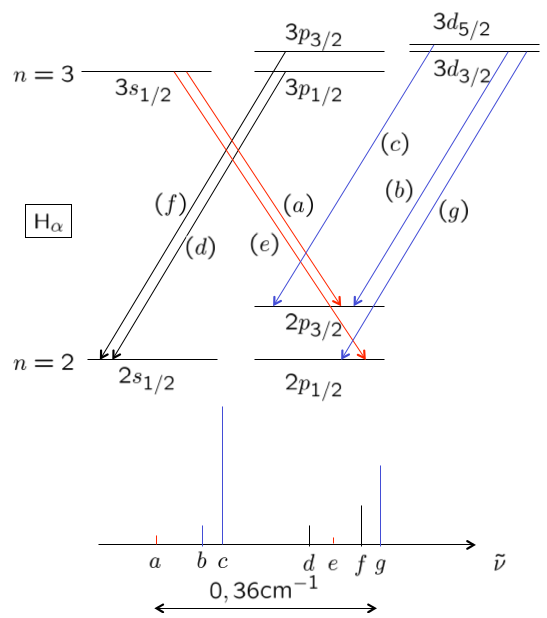
\includegraphics[scale=0.55]{ch1/image8.png}
	\captionof{figure}{ }
	\end{wrapfigure}
L'énergie $T$ transférée de 1 vers 2 s'obtient en explicitant $\Delta P_\perp^2$
\begin{equation}
T=\frac{\Delta P_\perp^2}{2m_2}\simeq \frac{2e_1^2e_2^2}{m_2v^2p^2}
\label{eq:1.ad}
\end{equation}
Le seul paramètre (aléatoire) dont dépend $T$ est le paramètre d'impact $p$. Ainsi, le nombre
de collisions caractérisés par un transfert d'énergie compris entre $T$ et $T+dT$ est caractérisé
par un paramètre d'impact entre $p$ et $p+dp$. Comme nous sommes en présence d'une géométrie
cylindrique, la particule incidente devra se trouver dans un anneau. La section efficace du 
projectile $d\sigma$ doit forcément être l'aire de cet anneau
\begin{equation}
d\sigma=2\pi pdp=\left|\frac{d(\pi p^2)}{dT}\right| dT
\label{eq:1.se}
\end{equation}
En calculant la dérivée de \eqref{eq:1.ad} dans l'expression \eqref{eq:1.se}, on trouve 
la forme de la section efficace de Rutherford pour la diffusion (scattering) coulombienne qui 
sera déduite bien plus tard (exactement) par la mécanique quantique.\ \\

\cadre{\begin{equation}
d\sigma \approx 2\pi\dfrac{e_1^2e_2^2}{m_2v^2}\dfrac{dT}{T^2}
\end{equation}}\ \\

\subsubsection{Résultats préliminaires}
Cette formule nous permet d'obtenir des résultats préliminaire pour le stopping et le 
straggling. Sachant que $S = \int Td\sigma$ et $W = \int T^2d\sigma$, on trouve
\begin{equation}
S\simeq 2\pi \frac{e_1^2e_2^2}{m_2v^2}\int_{T_{max}}^{T_{min}}\frac{dT}{T},\qquad\qquad
W\simeq 2\pi \frac{e_1^2e_2^2}{m_2v^2} \int_{T_{max}}^{T_{min}}dT
\end{equation}
Après intégration (à connaitre \textbf{par coeur}!)\ \\

\cadre{
\begin{eqnarray}
&&S\simeq 2\pi \frac{e_1^2e_2^2}{m_2v^2}\int_{T_{max}}^{T_{min}}\frac{dT}{T}\vspace{2mm}\\
&&W\simeq 2\pi \frac{e_1^2e_2^2}{m_2v^2} \int_{T_{max}}^{T_{min}}dT
\end{eqnarray}}\ \\

En utilisant le \textbf{nombre d'arrêt} (\textit{stopping number}) $\DS 
L=\frac{1}{2}\ln{\left(\frac{T_{max}}{T_{min}}\right)}$ on peut ré-écrire
\begin{equation}
S\simeq 4\pi \frac{e_1^2e_2^2}{m_2v^2}L
\end{equation}

\textsc{Résultats préliminaires pour le stopping}\ \\
Soit les électrons $(e)$ de la cible (densité $NZ_2$, masse $m$ et charge $-e$) et les 
noyaux $(n)$ de la cible (densité $N$, masse $M_2$ et charge $Z_2e$). On peut calculer 
l'énergie moyenne en multipliant $S_e$ par $NZ_2\Delta x$. En faisant de même pour $S_n$ :
\begin{eqnarray}
&&S_e=\frac{4\pi e_1^2e^2}{mv^2}L_e \Rightarrow  \langle \Delta E\rangle_e\simeq NZ_2\Delta x \times \frac{4\pi e_1^2e^2}{mv^2}L_e\vspace{2mm}\\
&&S_n=\frac{4\pi e_1^2Z_2^2e^2}{M_2v^2}L_n \Rightarrow  \langle \Delta E\rangle_n\simeq N\Delta x \times \frac{4\pi e_1^2Z_2^2e^2}{M_2v^2}L_n
\end{eqnarray}
Effectuons le rapport de ces deux dernières expressions
\begin{equation}
\frac{\langle \Delta E\rangle_n}{\langle \Delta E\rangle_e}\simeq \frac{m}{M_2}Z_2\frac{L_n}{L_e}
 {\mbox{~~or~~}} \frac{mZ_2}{M_2}<10^{-3}
\end{equation}
En laissant pour l'instant tomber le rapport des $L$ (straggling number), on obtient un terme 
inférieur à $10^{-3}$ : un électron incident va perdre beaucoup plus d'énergie lorsqu'il va 
interagir avec d'autres électrons plutôt qu'avec des neutrons.

\newpage
\subsubsection{Détermination de l'énergie transférée maximale $T_{max}$}
	\begin{wrapfigure}[8]{r}{3.5cm}
	\vspace{-5mm}
	\includegraphics[scale=0.75]{ch1/image9.png}
	\captionof{figure}{ }
	\end{wrapfigure}
Soit $T_{max}$, l'énergie cinétique maximale qui peut être transférée dans une collision. 
Celle-ci est obtenue pour $p=0$, soit quand la particule cible est le plus proche possible
de la particule incidente. Nous ne sommes plus ici dans le cadre du précédent modèle (\textit{
soft collision}) mais ce n'est pas grave car seule une limite maximale est recherchée. L'image
ci-contre représente le système du laboratoire.\\

Dans le système du centre de masse (désigné par un \textit{prim})
\begin{equation}
v_{CM}=\frac{m_1v}{m_1+m_2},\qquad\qquad\qquad v'=v-v_{CM}
\end{equation}
Considérons une collision élastique avec uniquement un transfert d'énergie cinétique. L'intérêt
d'une telle collision dans le système du centre de masse est que seule la direction change : 
la vitesse et le module restent inchangés.
\begin{center}
	\includegraphics[scale=0.75]{ch1/image10.png}
	\captionof{figure}{ }
\end{center}
La situation correspondant à un maximum d'énergie transférée correspond à celle où la variation 
de la direction est la pus importante, soit quand tout change de sens. Dans le système du 
laboratoire, la vitesse maximale $v_{2,max}$ de la particule 2 s'écrit
\begin{equation}
v_{2,max}=\frac{2m_1v}{m_1+m_2}
\end{equation}
L'énergie maximale transférée vaut donc
\begin{equation}
T_{max}=\frac{m_2v_{2,max}^2}{2}=\gamma E
\end{equation}
où $\DS\gamma=\frac{4m_1m_2}{(m_1+m_2)^2} {\mbox{~~~~et~~~~}}E=\frac{m_1v^2}{2}$.\\

Ceci mène directement à deux implications 
\begin{enumerate}
\item Pour $m_1=m_2 \to \gamma=1$ ; l'énergie transférée peut valoir toute l'énergie de la particule
incidente
\item Pour $m_1\ll m_2$ ou l'inverse $\to \gamma$ petit
\end{enumerate}
Il en vient que\\

\cadre{\begin{itemize}
\item[$\bullet$] Un grand transfert d'énergie est possible pour l'interaction $e^-/e^-$
\item[$\bullet$] Un petit transfert d'énergie est possible pour l'interaction ion$/e^-$
\item[$\bullet$] Un petit transfert d'énergie est possible pour l'interaction $e^-/$ion
\item[$\bullet$] Un petit transfert d'énergie est possible pour l'interaction ion/ion
\end{itemize}
Notons que l'on parle de transfert possible et \textbf{pas} de probabilité.}

\newpage
\subsubsection{Détermination de l'énergie transférée minimale $T_{min}$}
Nous allons calculer $T_{min}$ dans le cas d'une collision avec un $e^-$ (il s'agit du cas
pratique le plus intéressant). Pour un électron isolé et libre, on trouve $T_{min}=0$. Or, 
la section efficace de stopping contient le logarithme du rapport $T_{max}/T_{min}$, il y 
aura divergence. Deux façon de lever la divergence existent
\begin{enumerate}
\item Considérer que les $e^-$ sont liés à une molécule ou à un atome
\item Considérer l'écrantage de l'interaction de Coulomb
\end{enumerate}
La première solution sera retenue?. Le plus simple est le modèle simple de Thompson où 
$T_{min}$ est l'énergie d'excitation la plus faible. Néanmoins, on s'intéressera ici 
au modèle de Bohr, plus proche du résultat quantique.\\

La vision de Bohr revient à voir la matière comme une collection d'oscillateurs harmonique 
classiques. En cas de choc lent $(2\pi/\omega_0\ll \tau$), l'oscillateur peut directement 
se remettre en place et le transfert d'énergie est négligeable (invariance adiabatique). 
L'orbite de l'électron n'est que provisoirement déformée, les états initiaux et finaux sont
identiques.\\

Si par contre le temps d'interaction est court par rapport à la période de l'oscillateur 
($\tau \ll 2\pi/\omega_0$), l'oscillateur reçoit une impulsion $F\times\tau$. C'est ce que
nous considérons ici. En utilisant l'expression du temps d'interaction, on trouve un ordre
pour $T_{min}$
\begin{equation}
\frac{2p}{v}\ll\frac{2\pi}{\omega_0} \Rightarrow p_{max}\sim\frac{v}{\omega_0}
 \Rightarrow T_{min}\sim\frac{2e_1^2e^2\omega_0^2}{mv^4}
\end{equation}
avec $\DS T\simeq \frac{2e_1^2e_2^2}{mv^2p^2}$ et $p_{max}$, le 
\textit{rayon adiabatique de Bohr}.\\

On peut alors, dans le modèle de Bohr (en reprenant les précedentes expressions), calculer 
la section efficace de stopping électronique comme il n'y a plus divergence \\

\cadre{\begin{equation}
S_e=\frac{4\pi Z_2 e_1^2e^2}{mv^2}L_e\quad\text{avec}\quad L_e=\ln\frac{Cmv^3}{|e_1e
|\omega_0}{\mbox{~~et~~}}C\simeq 1
\end{equation}
où $L=\frac{1}{2}\ln{\left(\frac{T_{max}}{T_{min}}\right)}$ et $C$, une correction introduite 
par Bohr que nous ne prendrons pas en compte.}


\subsubsection{Déviation angulaire maximale}
Soit $m_2\leq m_1$. Soit à gauche le référentiel du laboratoire et à droite, celui du centre de 
masse
\begin{center}
	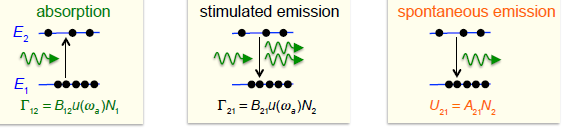
\includegraphics[scale=0.45]{ch1/image11.png}
	\captionof{figure}{ }
\end{center}
Dans le référentiel du centre de masse
\begin{equation}
v_{CM}=\frac{m_1}{m_1+m_2}v_{1i},\qquad\qquad\qquad v'=v-v_{CM}
\end{equation}
On en tire
\begin{equation}
v'_{1i}=v_{1i}-v_{CM}=\frac{m_2}{m_1+m_2}v_{1i}
\end{equation}
Comme nous avons une collision élastique dans le repère du centre de masse, seule la direction
est modifiée (et donc $v_{1f}'=v_{1i}'$)
\begin{equation}
v'_{1f}=\frac{m_2}{m_1+m_2}v_{1i}
\end{equation}

	\begin{wrapfigure}[8]{r}{5.5cm}
	\vspace{-5mm}
	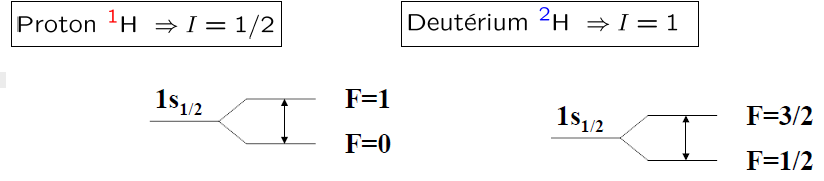
\includegraphics[scale=0.65]{ch1/image12.png}
	\captionof{figure}{ }
	\end{wrapfigure}

L'angle maximal $\theta_{max}$ est obtenu lorsqu'un angle droit est formé au niveau de la
circonférence du cercle. On choisit alors $v_{1f}'$ ($v_{CM}$) étant fixé de sorte à avoir
$\theta_{max}$. Après un peu de trigonométrie
\begin{equation}
\sin{\theta_{max}}=\frac{v'_{1f}}{v_{CM}}=\frac{m_2}{m_1}
\end{equation}
Si $m_2\geq m_1$, on trouve $\theta_{max}=\pi$. \\

En conclusion\\

\cadre{\begin{itemize}
\item[$\bullet$] Grandes déviations possibles ($\theta_{max}=\pi/2$) pour l'interaction $e^-/e^-$
\item[$\bullet$] Très grandes déviations possibles ($\theta_{max}=\pi$) pour l'interaction $e^-/$ion
\item[$\bullet$] Petites déviations pour l'interaction ion/$e^-$
\item[$\bullet$] Grandes déviations possibles (dépendant de $m_1$ et $m_2$) pour l'interaction ion/
ion
\end{itemize}}

\subsection{Conclusions à propos de ces considérations de base}
\subsubsection{Pour les ions incidents}
De façon générale les pertes électroniques dominent (petits transfert d'énergie et petites déviations
angulaires) et les pertes nucléaires (collisions noyaux) sont rares (se produisent pour un 
faible nombre de projectives mais de grand transferts d'énergies sont possibles ainsi que de 
grandes déviations angulaires). Ils ont une \textit{trajectoire rectilignes accompagnées de 
pertes d'énergie faibles et continues}.

\subsubsection{Pour les électrons incidents}
Les pertes électroniques dominent (mais cette fois grands transferts d'énergie et grandes déviations
angulaires possibles). On retrouve aussi des pertes nucléaires (petits transferts d'énergie mais
très grandes déviations angulaires possibles (possibilité de rétro-diffusion). Ils ont une 
\textit{trajectoire courbée accompagnée de grandes pertes d'énergie}.






\chapter{Interaction des ions avec la matière}
	\begin{wrapfigure}[11]{l}{10.5cm}
	\vspace{-5mm}
	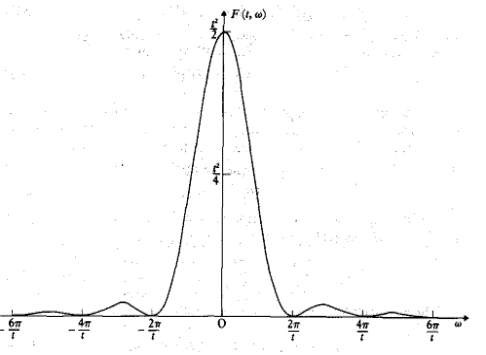
\includegraphics[scale=0.3]{ch2/image1.png}
	\captionof{figure}{ }
	\end{wrapfigure}
Ci-contre, à gauche, sont représenté les trajectoires de particules $\alpha$ d'une énergie
de 5.5 MeV. On observe que trois d'entre-elles sont rentrées en collisions avec les noyaux
(déviation angulaire plus importante). A droite, considérons un proton incident sur 
de l'aluminium, décrit par le modèle de Bohr. Ce modèle étant classique, il ne peut pas être
correct dans la zone relativiste. Lorsque la vitesse du projectile se rapproche de $v_0$, 
la vitesse de Bohr\footnote{On associe l'énergie à une certaine vitesse via l'énergie cinétique.}, 
on ne peut plus considérer que la particule est au repos, le modèle n'est dès lors plus 
valable\footnote{L'hypothèse de Bohr est telle que la particule cible est au repos.}

\section{Modèle semi-classique du pouvoir d'arrêt électronique}
Un rappel sur les oscillateurs classiques et l'approximation dipolaire est faite dans les
slides 5 à 12 : n'étant que des rappels/pré-requis, ils ne sont pas repris ici.

\subsection{Vitesses intermédiaires : $v_0\ll v \ll c$}
Dans le modèle semi-classique de \textsc{Bethe} (\textit{1930}), le noyau est traité 
classiquement et les électrons quantiquement, ils ne sont plus traités comme des oscillateurs
classiques. On s'intéresse ici au cas ou le modèle de Borh est correct. \\

Considérons un atome cible avec $Z_2$ électrons (masse $m$) et les états stationnaires $\ket j$ 
d'énergie $\epsilon_j$ où $j$ est un nombre quantique tel que $j=0$ dénote l'état fondamental. 
Les fréquences de résonance pour un atome dans son état initial sont données par
\begin{equation}
\hbar\omega_{j0}=\epsilon_j-\epsilon_0
\end{equation}
On dira que les électrons sont au repos durant l'interaction si $v\gg v_0$.
\\

Pour une énergie $Q$ perdue par l'ion incident, \textsc{Bethe} a posé
\begin{equation}
S=\sum_j\int Q d\sigma_Rf_{j0}(Q)
\end{equation}
où $\sigma_R$ est la section efficace de \textsc{Coulomb} pour un transfert d'énergie $Q$ 
(où $R$ pour \textsc{Rutherford}) et $f_{j0}$ sont les \textit{forces d'oscillateur généralisées}
qui incluent tous les effets quantiques pour la section efficace d'arrêt : ils décrivent les 
probabilités de transition entre les états pour une énergie transférée $Q$ donnée.\\

Afin de déterminer l'expression de $f_{j0}$, résolvons l'équation de Schrödinger dépendante du 
temps (celle-ci gouverne le mouvement électronique)
\begin{equation}
(H+V)\Psi(\overrightarrow{r},t)=i\hbar \frac{d\Psi(\overrightarrow{r},t)}{dt}
\end{equation}
où $H$ est l'hamiltonien d'un atome isolé de la cible, $\Psi(t)$ la fonction d'onde d'un état
lié et $V$ le potentiel décrivant l'interaction avec le projectile donné par
\begin{equation}
V(\overrightarrow{r},t)=\sum_{\nu=1}^{Z_2}\frac{-e_1e}{\overrightarrow{r}_\nu-\overrightarrow{R}(t)}
\end{equation}
où $\vec r = (\vec{r}_1,\dots \vec{r}_{Z_2})$ représente la trajectoire du projectile avec 
$\vec r_\nu$ l'opérateur position du $\nu^e$  électron et $\vec{R}=\vec{p}+\vec{v}t$. Développons
$\Psi(t)$ sur la base formée des états stationnaires
\begin{equation}
\Psi(\overrightarrow{r},t)=\sum_{j}c_j(t)e^{-i\epsilon_jt}|j\rangle
\end{equation}
où $\ket j$ sont les solutions de $H\ket j = \epsilon_j\ket j$. Dans le cadre de la méthode des
perturbations au premier ordre, on peut développer les coefficients $c_j$ en puissance du 
potentiel perturbatif $V$
\begin{equation}
c_j(t) = \delta_{j0} + c^{(1)}_j(t) + c^{(2)}_j(t) + \dots
\end{equation}
avec $\delta$ le symbole de Kronecker et

\begin{eqnarray}
c_j^{(1)}(t)=\frac{1}{i\hbar}\int_{-\infty}^{t}dt'e^{i\omega_{j0}t'}\langle j|V(\overrightarrow{r},t')|0\rangle\\
c_j^{(2)}(t)= \left(\frac{1}{i\hbar}\right)^2\sum_k\int_{-\infty}^{t}dt'e^{i\omega_{jk}t'}\langle j|V(\overrightarrow{r},t')|k\rangle
\times \int_{-\infty}^{t'}dt''e^{i\omega_{k0}t''}\langle k|V(\overrightarrow{r},t'')|0\rangle
\end{eqnarray}
et ainsi de suite mais ici nous ne nous intéressons que aux coefficients $c_j^{(1)}(\infty)$ car
seul le premier ordre nous intéresses. Ceux-ci représentent les amplitudes de transition. 
Substituons $c_j^{(1)}(\infty)$ dans l'expression explicite du potentiel, prenons-en la 
transformée de \textsc{Fourier} et intégrons sur $t'$
\begin{equation}
c_j^{(1)}(\infty)=\frac{-e_1e}{i\pi\hbar}\int \overrightarrow{dq}\frac{e^{-i\overrightarrow{q}.\overrightarrow{p}}}{q^2}F_{j0}(\overrightarrow{q})\delta(\omega_{j0}-\overrightarrow{q}.\overrightarrow{v})
\end{equation}
où $\DS F_{j0}(\overrightarrow{q})=\left\langle j\left| \sum_{\nu=1}^{Z_2}e^{i\overrightarrow{q}.\overrightarrow{r_\nu}}\right| 0\right\rangle$. Notons $Q=\frac{\hbar^2q^2}{2m}$. Par le 
\textsc{Postulat IV} de la mécanique quantique, les probabilités de transitions sont données 
par
\begin{equation}
P_j(p)=\left| \langle j| \Psi(\infty)\rangle\right|^2
\end{equation}
Ce qui donne dans le cadre de la méthode des perturbations au premier ordre
\begin{equation}
P_j(p)=\left| c_j^{(1)}(\infty)\right|^2
\end{equation}
Pour que $c_j^{(1)}(\infty) \neq 0$ pour $\omega_{j0} < q\nu$, il faut que (condition sur $Q$)
\begin{equation}
\omega_{j0}^2<q^2v^2 \Rightarrow 2mv^2Q>(\epsilon_j-\epsilon_0)^2
\end{equation}

\subsubsection{Approximation des collisions distantes - Approximation dipolaire}
Afin d'obtenir notre expression de $f_{j0}$, nous allons devoir utiliser une approximation. 
Considérons $c_j^{(1)}(\infty)$ à grand $p$ (\textit{collisions distantes}). Par l'approximation
dipolaire
\begin{equation}
e^{i\overrightarrow{q}.\overrightarrow{r}}\simeq 1+i\overrightarrow{q}.\overrightarrow{r}
\end{equation}
On obtient donc
\begin{equation}
F_{j0}(\overrightarrow{q})\simeq i\overrightarrow{q}\left\langle j\left| \sum_{\nu=1}^{Z_2}\overrightarrow{r_\nu}\right| 0\right\rangle
\end{equation}
En choisissant l'axe $x$ selon la vitesse du projectile et l'axe $y$ selon le paramètre 
d'impact, on voit apparaître des fonctions de \textsc{Bessel} modifiée $K_{0,1}$, d'ordre 0 et 1
\begin{equation}
c_j^{(1)}(\infty)=-\frac{2e_1e\omega_{j0}}{i\hbar v^2}\left\langle j\left| \sum_{\nu}^{Z_2}\overrightarrow{r}_\nu \right|0\right\rangle
 \times\left(iK_0\left(\frac{\omega_{j0}p}{v}\right),K_1\left(\frac{\omega_{j0}p}{v}\right),0\right)
\end{equation}
Les probabilités de transitions deviennent donc (données par $|c_j|^2$)
\begin{equation}
P_j(p)=-\frac{2e_1^2e^2Z_2}{mv^2p^2\hbar\omega_{j0}}f_{j0}
 \times\left\{\left[\frac{\omega_{j0}p}{v}K_0\left(\frac{\omega_{j0}p}{v}\right)\right]^2+\left[\frac{\omega_{j0}p}{v}K_1\left(\frac{\omega_{j0}p}{v}\right)\right]^2\right\}
\end{equation}
La grandeur $f_{j0}$ est appelée la \textbf{force d'oscillateur dipolaire} et a comme
expression
\begin{equation}
f_{j0}=\frac{2m}{3\hbar^2Z_2}(\epsilon_j-\epsilon_0)\left|\left\langle j\left|\sum_{\nu}^{Z_2}\overrightarrow{r}_\nu\right|0\right\rangle\right|^2
\end{equation}
Avec la règle de somme de \textsc{Thomas-Reiche-Kuhn} $\sum_j f_{j0}=1$.

\subsubsection{Comparaison modèle classique et semi-classique}
Maintenant que nous avons la probabilité d'une transition, il nous faut l'énergie moyenne. 
Considérons l'énergie transférée moyenne $T_{moy}$
\begin{equation}
T_{moy}(p)=\sum_jP_j(p)\hbar\omega_{j0}
\end{equation}
Comparons cette expression avec le résultat classique donné par 
\begin{equation}
T= \frac{2e_1^2e^2}{mv^2p^2}f_{dist}(p),\qquad\text{ où }\quad 
f_{dist}(p)=\left[\frac{\omega_{0}p}{v}K_0\left(\frac{\omega_{0}p}{v}\right)\right]^2+\left[\frac{\omega_{0}p}{v}K_1\left(\frac{\omega_{0}p}{v}\right)\right]^2
\end{equation}
Les expressions sont identiques à condition que
\begin{equation}
f_{dist}(p)=\sum_jf_{j0}\left[\frac{\omega_{j0}p}{v}K_0\left(\frac{\omega_{j0}p}{v}\right)\right]^2+\left[\frac{\omega_{j0}p}{v}K_1\left(\frac{\omega_{j0}p}{v}\right)\right]^2
\end{equation}
Pour généraliser les fonctions $f_{j0}$ que nous venons d'élaborer aux grandes valeurs de $Q$, 
\textsc{Bethe} a posé
\begin{equation}
f_{j0}(Q)=\frac{1}{Z_2}\frac{\epsilon_j-\epsilon_0}{Q}|F_{j0}(\overrightarrow{q})|^2
\end{equation}
Avec cette forme la, lorsque $Q$ est petit, on retrouve l'expression que nous venons de calculer
\begin{equation}
f_{j0}(Q)\big\vert_{Q\simeq 0}=f_{j0}
\end{equation}

\subsubsection{Pouvoir d'arrêt : formule de Bethe}
Il est nécessaire de faire la distinction entre les collisions distantes ou proche (via $p$), soit 
les collision avec une grande ou petite quantité de mouvement transférée (via $q$) ou encore 
les collisions avec une grande ou petite énergie transférée (via $Q$). Pour se faire, 
nous allons séparer l'intégrale suivante en deux parties par rapport à $Q_0$
\begin{equation}
S=\sum_j\int Q d\sigma_Rf_{j0}(Q)
\end{equation}
$\bullet$ Pour $Q<Q_0$, l'approximation dipolaire est valide ($Q_0$)
\begin{equation}
S_{dist}=\sum_jf_{j0}\int_{(\epsilon_j-\epsilon_0)^2/2mv^2}^{Q_0} Q d\sigma_R
\end{equation}

$\bullet$ Pour $Q>Q_0$, il faut déterminer la borne supérieure de l'intégrale. On considère que 
la masse d'un ion $m_1\gg m$, la masse d'un électron.
\begin{equation}
T_{max} = \gamma E = \frac{4m_1m}{(m_1+m)^2}\frac{m_v^2}{2} \approx 2mv^2
\end{equation}
où nous avons négliger $m$ par rapport à $m_1$. On trouve alors la section efficace 
d'arrêt suivante
\begin{equation}
S_{proche}=\int_{Q_0}^{2mv^2} Q d\sigma_R\sum_jf_{j0}(Q)
\end{equation}
\textsc{Bethe} a démontré que
\begin{equation}
\sum_jf_{j0}(Q)=1
\end{equation}
Nous avons alors
\begin{equation}
S_{proche}=\int_{Q_0}^{2mv^2} Q d\sigma_R\equiv \sum_jf_{j0}\int_{Q_0}^{2mv^2} Q d\sigma_R
\end{equation}
En sommant les collisions proches et distantes, on trouve finalement
\begin{equation}
S=S_{proche}+S_{dist}= \sum_jf_{j0}\int_{(\epsilon_j-\epsilon_0)/2mv^2}^{2mv^2} Q d\sigma_R
\end{equation}
En considérant l'expression explicite $d\sigma_R= 2\pi \frac{e_1^2e_2^2}{m_2v^2}\frac{dQ}{Q^2}$, 
on obtient
\begin{equation}
S=\frac{4\pi e_1^2e^2}{mv^2}Z_2\sum_jf_{j0}\ln{\frac{2mv^2}{\epsilon_j-\epsilon_0}}
\end{equation}
La formule du pouvoir d'arrêt de \textsc{Bethe} se note généralement\\

\cadre{\begin{equation}
S_{e}=\frac{4\pi e_1^2e^2}{mv^2}Z_2\ln{\frac{2mv^2}{I}}
\end{equation}
où $I$ est définie comme l'énergie moyenne d'excitation telle que $\ln I=\sum_j f_{j0}\ln{
(\epsilon_j-\epsilon_0)}$. Ceci n'est valable que \textbf{si} $m_1\gg m, v\gg v_0 \to mv^2 \gg
 \hbar \omega_0$.}\ \\
 
On peut facilement comparer le modèle de \textsc{Bethe} à celui de \textsc{Bohr} via 
\begin{equation}
S_e=\frac{4\pi Z_2 e_1^2e^2}{mv^2}L_e
\end{equation}
où 
\begin{equation}
L_e=\ln\frac{Cmv^3}{|e_1e|\omega_0}
\end{equation}
pour le \textsc{Bohr} et 
\begin{equation}
L_e=\ln{\frac{2mv^2}{I}}
\end{equation}
pour \textsc{Bethe}.

\subsubsection{Dépendances principales du pouvoir d'arrêt}
Le pouvoir d'arrêt se compose lui-même de trois dépendances\ \\

\retenir{\begin{equation}
-\left( \frac{dE}{dx}\right)_{elec}=NS_{e}=\frac{4\pi e_1^2e^2}{mv^2}NZ_2\ln{\frac{2mv^2}{I}}
\end{equation}}\ \\

Les dépendances sont les suivantes
\begin{enumerate}
\item $\frac{4\pi e_1^2e^2}{mv^2}\Rightarrow{\mbox{D\'ependance principale dans la vitesse}}$, plus la vitesse augmente, plus le pouvoir d'arrêt diminue.
\item $NZ_2\Rightarrow{\mbox{D\'ependance principale dans le mat\'eriau}}$, plus il est grand, plus le pouvoir augmente.
\item $\ln{\frac{2mv^2}{I}}\Rightarrow{\mbox{D\'ependance faible dans la vitesse et dans le mat\'eriau}}$
\end{enumerate}

	\subsubsection{Énergies moyenne d'excitation}
	\begin{wrapfigure}[7]{r}{6.5cm}
	\vspace{-5mm}
	\includegraphics[scale=0.5]{ch2/image2.png}
	\captionof{figure}{ }
	\end{wrapfigure}
	

L'énergie moyenne d'excitation $I$ ne dépend \textbf{que} du matériau et \textbf{pas} du 
projectile. Il est possible de le calculer mais tout le monde s'en fiche car on peut l'obtenir
expérimentalement\footnote{De plus, comme il intervient dans $\log S$ il n'est pas nécessaire
de connaître sa valeur avec précision} via des formules empiriques. Celui-ci varie approximativement
linéairement (les irrégularités sont dues à la structure en couches de l'atome) avec $Z$ :
\textit{modèle de l'atome de Thomas-Fermi} où les électrons atomiques forment un gaz.

\newpage
\subsection{Grandes vitesses - Équation de \textsc{Bethe-Bloch} : $v_0<v\approx c$}
\textsc{Bloch} a apporté de nombreuses corrections à l'équation de \textsc{Bethe} pour 
former l'équation de \textsc{Bethe-Block}\\

\cadre{\begin{equation}
S_e = \dfrac{4\pi r_e^2mc^2}{\beta^2}Zz^2L(\beta)
\end{equation}
où $\DS L(\beta)= L_0(\beta) = \frac{1}{2}\ln\left(\frac{2mc^2\beta^2W_m}{1-\beta^2}\right)
-\beta^2-\ln I-\frac{C}{Z}-\frac{\delta}{2}$.}\ \\

Il s'agit en réalité de la même équation mais notée différemment, toute la différence se 
trouve dans le \textit{stopping number} $L$ qui contient donc les termes correctifs. 
Intéressons-nous à ceux-ci
\begin{itemize}
\item[$\bullet$] \textit{Corrections dues aux collisions}\ \\
$W_m$ donne l'énergie maximale transférée en une collision à un électron
libre\footnote{Il s'agit d'une expression relativiste non-approchée}
\begin{equation}
W_m=\frac{2mc^2\beta^2}{1-\beta^2}\left[1+\frac{2m}{m_1(1-\beta^2)^{1/2}}+\left(\frac{m}{m_1}\right)^2\right]^{-1}
\end{equation}
Pour $m_1\gg m$, on retrouve bien $2m\gamma_1^2v^2$.
\item[$\bullet$] \textit{Corrections relativistes}\ \\
Si $v\approx c$, il faut apporter des corrections relativistes. Lorsque l'on travaille avec
des vitesses relativistes, il faut considérer des électrons de plus en plus lointain ce qui, 
forcément, augmente le pouvoir d'arrêt. En effet, $p_{max} \propto \gamma_1v/\omega_0$ ce qui
montre que le paramètre d'impact augmente lorsque la vitesse fait de même. Le calcul relativiste
classique du champ donne
\begin{equation}
\overrightarrow{E}(\omega)=-\frac{e_1\omega}{\pi \gamma_1v^2}\left(\frac{i}{\gamma_1}K_0\left(\frac{\omega_{j0}p}{\gamma_1v}\right),K_1\left(\frac{\omega_{j0}p}{\gamma_1v}\right),0\right)
\end{equation}
On y voit apparaître des $\gamma_1$ et $f(p)$ se voit modifiée par ce fameux terme
\begin{equation}
f_{dist}(p)=\frac{1}{\gamma_1^2}\left[\frac{\omega_{0}p}{\gamma_1v}K_0\left(\frac{\omega_{0}p}{\gamma_1v}\right)\right]^2+\left[\frac{\omega_{0}p}{\gamma_1v}K_1\left(\frac{\omega_{0}p}{\gamma_1v}\right)\right]^2
\end{equation}
La composante principale en la vitesse se voit modifiée
\begin{equation}
\frac{4\pi e_1^2e^2}{mv^2}\Rightarrow \frac{4\pi e_1^2e^2}{m\gamma_1^2v^2}=\frac{4\pi e_1^2e^2}{mv^2}(1-\beta^2)
\end{equation}
où le $(1-\beta^2)$ apparaissant permet de comprendre le terme correspondant dans la formule de 
\textsc{Bethe-Bloch}, il va être possible de lui donner un sens physique. Sachant que la quantité 
de mouvement de la particule incidente devient $m\gamma_1v$, on en tire
\begin{equation}
T_{max}=2m\gamma_1^2v^2
\end{equation}
La composant logarithmique se modifie selon
\begin{equation}
\ln{\frac{2mv^2}{I}}\Rightarrow \ln{\frac{2m\gamma_1^2v^2}{I}}=\ln{\frac{2mv^2}{I(1-\beta^2)}}
\end{equation}
La combinaison de toutes ces relations implique donc que le pouvoir d'arrêt augmente lorsque 
la vitesse augmente, ce qui est la conséquence du traitement relativiste. 
\end{itemize}

\newpage

\begin{itemize}
\item[$\bullet$] \textit{Correction de densité}\ \\
Le terme correspondant à ces corrections est le $-\delta/2$. La formule de \textsc{Bethe} est 
valable pour un gaz de faible densité (atomes isolés) mais pour un solide il faut tenir compte
des effets collectifs d'un grand nombres d'atomes : on peut utiliser le modèle de Fermi. Une 
particule chargée incidente va polariser le milieu. Le champ électrique induit va alors donner un
moment dipolaire électrique aux atomes et il en résultera un champ électrique opposé à celui 
produit par la particule chargée. Le champ électrique sera donc réduit via l'écrantage des dipôles.\\

A cause de cette diminution du champ (à cause de la polarisation), les atomes lointains ont un 
effet plus faible. L'effet de densité apparaît surtout aux grandes vitesses, en même temps que les 
effets relativiste (ils vont se "compenser"). S'il n'est signifiant qu'aux énergies élevées c'est 
à cause du facteur $\gamma_1$ présent dans $p_{max}$ qui augmente l'erreur commise en ignorant la
polarisation du milieu : si $v$ augmente, $p_{max}$ augmente et donc $\delta/2$ augmente causant une
diminution de $S$.

\begin{center}
	\includegraphics[scale=0.5]{ch2/image3.png}
	\captionof{figure}{L'effet relativiste et de densité vont se stabiliser de sorte que le 
	pouvoir d'arrêt devient constant. On parle alors de \textit{plateau de Fermi}, constant à
	grande vitesse.}
\end{center}

On peut écrire la correction de densité
\begin{equation}
\frac{\delta}{2}=\ln{\frac{\hbar\omega_p}{I}}+\ln{\gamma_1\beta}-\frac{1}{2}
\end{equation}
avec $\omega_p=\sqrt\frac{ne^2}{\epsilon_0m}$ la \textit{pulsation plasma}, mais ceci est plus
informatif.

\item[$\bullet$] \textit{Correction shell} ("en couches")\ \\
Il s'agit du terme $-C/Z$. Nos deux formules sont basées sur l'hypothèse que $v\gg v_0$ (permet
de calculer $I$ moyen). Lorsque que n'est plus le cas, on ne peut plus considérer que tous les
électrons ont la même énergie de liaison. Le problème est que certains électrons sont plus liés 
que d'autres. Comme ils seront plus durs à arracher, leur contribution au pouvoir d'arrêt va 
diminuer et il ne faudra plus les considérer. On ajoute ainsi un terme de correction "moyen" qui
réduit $S$ de maximum 6\% qui ne dépend que de la vitesse et du matériau considéré, peu importe 
les couches. Il existe deux méthodes pour calculer $C/Z$
	\begin{enumerate}
	\item Une basées sur les fonctions d'ondes hydrogénoïdes (HWF)\footnote{Un électron interne ne
	 peut
	 pas être représenté par une fonction d'onde de la sorte mais comme la rigueur absolue n'est 
	 pas possible en s'en contentera car \textit{au moins} on a un résultat, bien que moins 
	 rigoureux.}
	\item Une basée sur l'approximation en densité locale (LDA)
	\end{enumerate}
	
%\begin{center}
\hspace{-1cm}	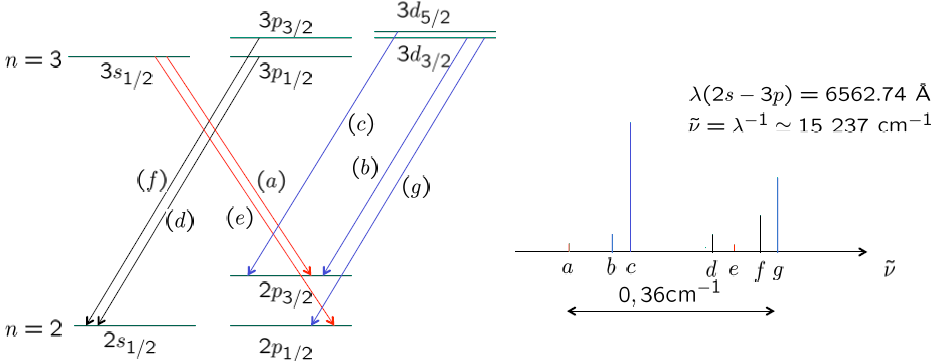
\includegraphics[scale=0.4]{ch2/image4.png}
	\captionof{figure}{A gauche la comparaison théorie/expérience (relativement bonne et comme la
	correction est logarithmique on s'en contentera), au centre le calcul par la méthode LDA et à
	droite selon HWF. L'écart entre les méthodes est plus grand pour des $Z$ élevés mais 
	les deux sont globalement assez bonnes.}
%\end{center}
\end{itemize} \ \\

Il est possible d'aller encore plus loin et de considérer des corrections au-delà de l'approximation
de \textsc{Born} au premier ordre.  On va considérer des vitesses toujours plus grande que $v_0$ mais
très proche de celle-ci de sorte que l'approximation de Born n'est plus valable\footnote{Il faut 
en effet que $v\gg v_0$ pour que $L_0$ soit valable}.Il faut rajouter des termes correctifs à 
$L_0$ qui apparaissent lors d'un développement de $L$ en puissance de $z$\ \\

\cadre{\begin{equation}
L(\beta) =  L_0(\beta) + zL_1(\beta) + z^2L_2(\beta)
\end{equation}}\ \\

Passons à nouveau en revue les différentes corrections
\begin{itemize}
\item[$\bullet$] \textit{Correction de Barkas-Andersen}\ \\
Il s'agit du terme $zL_1(\beta)$. Il s'agit d'une proportionnalité à une puissance impaire de la 
charge. Si la charge est positive, cela attire le nuage d'électrons et il y aura plus d'interactions :
augmentation du pouvoir d'arrêt. Si la charge est négative, les électrons sont repoussés et le 
pouvoir d'arrêt diminue. $S$ diffère donc entre les particules et antiparticules.
\begin{center}
	\includegraphics[scale=0.5]{ch2/image5.png}
	\captionof{figure}{Protons et antiprotons incidents sur une cible de silicium : le pouvoir 
	d'arrêt est plus important pour les protons que pour des antiprotons.}
\end{center}
\item[$\bullet$] \textit{Correction de Bloch}\ \\
Il s'agit du terme $z^2L_2(\beta)$, une correction pas très importante que l'on évalue généralement
avec l'évaluation de \textsc{Bichsel}
\begin{equation}
z^2L_2(y) = -y^2[1.202-y^2(1.042-0.855y^2+0.343y^4)]
\end{equation}
où $y=z\alpha/\beta$ avec $\alpha = 1/137$ le constante de structure fine.
\end{itemize}

\newpage
	\begin{wrapfigure}[11]{r}{9cm}
%	\vspace{-5mm}
	\includegraphics[scale=0.4]{ch2/image6.png}
	\captionof{figure}{ }
	\end{wrapfigure}
Évaluons maintenant les effets des différentes corrections. Le graphique ci-contre (à gauche) 
concerne des protons incidents sur une cible d'aluminium. On peut y voir que la correction de
\textsc{Bloch} (en bas à gauche) est vraiment très faible. A droite est représenté la correction
relative pour des protons incidents sur une cible d'or ($L_1$ concerne \textsc{Barkas} et $L_2$
\textsc{Bloch}).


\subsection{Petites vitesses}
Lorsque $v \lesssim v_0$, on ne peut plus appliquer la méthode des perturbations et il faut 
commencer à prendre en compte les captures électroniques par l'ion indicent (l'ion va si
lentement qu'il peut capturer un (ou plusieurs) électron) modifiant la charge $z^*$ de 
celui-ci. Par la théorie de \textsc{Thomas-Fermi}
\begin{equation}
z^*=z\left(1-e^{-v/(z^{2/3}v_0)}\right)
\end{equation}
Une technique consiste à considérer un état de charge moyen même si ce n'est pas vrai en tout 
point.


\section{Pouvoir d'arrêt nucléaire (faibles vitesses)}
Les effets étant tellement négligeable que nous ne rentrerons pas dans les détails ici. Comme
vu au premier chapitre, les collisions nucléaire pour des ions incidents sont rares et contribuent
peu au pouvoir d'arrêt total. Elle se produise presque exclusivement pour des ions incidents de 
faible vitesse et même alors leur contribution est faible. Cependant, elle peuvent avoir des effets
à postériori et causer des dégâts radiatifs.\\

	\begin{wrapfigure}[12]{r}{5.6cm}
	\vspace{-11mm}
	\includegraphics[scale=0.34]{ch2/image7.png}
	\captionof{figure}{ }
	\end{wrapfigure}
Plaçons-nous dans le système du centre de masses pour observer la diffusion par un angle 
$\theta$ due à un potentiel central $V(r)$. Reprenons la formule générale pour la section efficace
d'arrêt 
\begin{equation}
S_n = \int Td\sigma = \int T 2\pi p dp = 2\pi\gamma E\int \sin^2(\theta/2)pdp
\end{equation}
où $\gamma = \frac{4m_1m_2}{(m_1+m_2)^2}$. Pour le calculer, il est nécessaire de connaître $\theta$
ce qui peut se faire avec le schéma avec une particule incidente et cible représenté ci-contre.\\

Pour évaluer $\theta$, on utilise l'équation de la variation angulaire en coordonnée sphérique tout
en introduisant le potentiel. 

\begin{eqnarray*}
\frac{m_0}{2}\left[ \left( \frac{dr}{dt}\right)^2+r^2\left( \frac{d\varphi}{dt}\right)^{2}\right]+V(r)=\frac{m_0}{2}v^2\equiv E_r\\
m_0r^2\frac{d\varphi}{dt}=-m_0pv
\end{eqnarray*}
On en tire
\begin{equation}
\theta=\pi-2\int_{r_{m}}^\infty dr \frac{p}{r^2}\left( 1-\frac{V(r)}{E_r}-\frac{p^2}{r^2}\right)^{-1/2}
\end{equation}


Il faut maintenant spécifier le potentiel. Le plus logique serait d'utiliser celui de \textsc{Coulomb}
mais sa variation en $1/r$ cause une divergence du paramètre d'impact à cause de la portée infinie. 
Comme il y a toujours interaction, on va préférer considérer un effet d'écrantage par les électrons
atomiques qui diminue la portée du potentiel. Pour se faire, on va simplement introduire une 
exponentielle décroissante $\exp(-r/r_s)$.\\

Pour un modèle plus précis, on peut insérer une fonction $F_s(r/r_s)$. Le potentiel d'interaction 
devient alors
\begin{equation}
V(r)=\frac{z_1Z_2e^2}{r}F_s(\frac{r}{r_s})
\end{equation}
Il s'agit de la \textit{fonction d'écrantage universelle}, obtenue par ajustement aux résultats 
expérimentaux.\\

	\begin{wrapfigure}[12]{r}{5.6cm}
	\vspace{-11mm}
	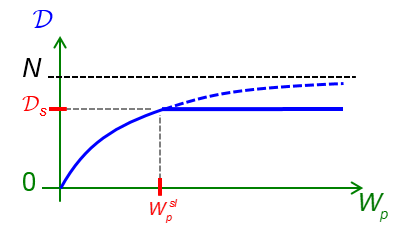
\includegraphics[scale=0.34]{ch2/image8.png}
	\captionof{figure}{ }
	\end{wrapfigure}
Mettons maintenant ces effets ensemble en considérant des protons incidents sur une cible 
d'aluminium comme représenté ci-contre. Nous avons $S = S_{elec} + S_{nucl} \approx S_{elec} 
= S_{coll}$. On voit que l'effet du pouvoir d'arrêt nucléaire est très faible, on retrouve
le plateau de Fermi à grande vitesse et une pente ou la formule de \textsc{Bohr} est valable.


\section{Pouvoir d'arrêt massique électronique et influence de la phase}
Par définition, le pouvoir d'arrêt massique d'un matériau est le rapport du pouvoir d'arrêt 
linéique et de lamasse volumique $\rho$ de ce matériau (unités usuelle : MeV.cm$^2$.g$^{-1}$. 
\begin{equation}
\frac{NS(E)}{\rho}=-\frac{1}{\rho}\frac{dE}{dx}
\end{equation}
Comme $\rho = M_AN/N_A$ où $M_A=AM_u$, en divisant des deux côtés par cette même quantité on 
trouve\\

\cadre{\begin{equation}
-\dfrac{1}{\rho}\dfrac{dE_{elec}}{dx} = 4\pi r_e^2mc^2\frac{N_A}{M_u}\dfrac{Z}{A}\dfrac{z^2}{\beta^2}
L(\beta)
\end{equation}}\ \\

Passons en revue les quatre facteurs du pouvoir d'arrêt massique électronique
\begin{enumerate}
\item Le facteur constant $4\pi r_e^2mc^2N_A/M_u = 0.307$ MeV.cm$^2$.g$^{-1}$ qui donne l'ordre
de grandeur de ce pouvoir
\item Le facteur $Z/A$ compris entre 0.4 et 0.5 pour tout les isotopes stable (sauf $H$). Comme
c'est le terme principal de dépendance du matériau et que celui-ci est $\pm$ constant la dépendance
du matériau est faible : c'est l'intérêt de cette formule
\item Le facteur $\beta^{-2}$ est une fonction monotone décroissante de la vitesse de l'ion qui
tend vers 1 pour les grandes énergies. Ce-dernier explique la diminution du pouvoir d'arrêt 
avec l'énergie. 
\item Le nombre d'arrêt $L(\beta)$ est une fonction monotone croissante (lente) de la vitesse 
et de $Z$.
\end{enumerate}

\subsection*{Influence de la phase}
Aux grandes énergies, la correction de densité influe impliquant une grande correction de phase 
dans les solides et faible dans les gaz. Aux faibles énergies il faut tenir compte de l'influence
des liaisons chimiques et intermoléculaires ce qui se traduit par une modification de la
valeur de $I$.

\section{Parcours et courbe de Bragg} 
\subsection{Parcours}
Lorsque les particules \textbf{chargées} perdent leur énergie dans la matière, elles parcourent une
certaine distance dans la matière mais celle-ci peut être variable a cause des pertes d'énergies 
et des déviations aléatoires (\textit{starggling}). Il faut alors définir plusieurs parcours
\begin{itemize}
\item[$\bullet$] Le parcours $R$ d'une particule chargée d'énergie $E$ dans un milieu et 
la valeur moyenne $\langle l \rangle$ de la longueur $m$ de sa trajectoire suivie jusqu'à son 
arrêt (en négligeant le mouvement thermique)
\item[$\bullet$] Le parcours projeté $R_p$ d'une particule chargée d'énergie $E$ dans un milieu. 
Celui-ci correspond à la valeur moyenne de sa profondeur de pénétration $\langle d \rangle$ dans la
direction initiale de la particule.
\end{itemize}
A cause du caractère sinueux des trajectoires, $R_r<R$. On défini alors le \textbf{facteur de détour}
$R_p/R_{CSDA} < 1$.\\

Dans l'approximation $CSDA$
\begin{equation}
R_{CSDA}=\int^{E}_{0}\frac{dE'}{NS(E')}
\end{equation}
En remplaçant $S$ par l'expression de \textsc{Bethe} (non-relativiste, avec $dE=Mv$d$v$)
\begin{equation}
R_{CSDA}\propto \int^{v}_{0}\frac{v^3dv}{L(v)}
\end{equation}
En négligeant la dépendance en la vitesse du nombre d'arrêt 
\begin{equation}
R_{CSDA}\propto v^4\propto E^2
\end{equation}
En réalité, l'équation de \textsc{Bethe} (ou \textsc{Bethe-Bloch}) n'est pas valable à faibles
vitesses et il faut nécessairement passer par de faibles vitesses pour s'arrêter. On utilisera 
alors la formule empirique suivante
\begin{equation}
\rho R_{CSDA}=\frac{E^{1.77}}{415}+\frac{1}{670}
\end{equation}

\subsubsection{Considérations sur le parcours}
Reprenons l'approximation $NS(E)\propto 1/E$. Soit une particule incidente de masse $M_i$ et de
charge $z_i$
\begin{equation}
NS(E)=-\frac{dE}{dx} \Rightarrow -\frac{M_i}{z_i^2}\frac{dv^2}{dx}\propto \frac{1}{v^2}
\end{equation}
Pour deux particules incidentes $(M_1,z_1)$ et $(M_2, z_2)$ de même vitesse initiale
\begin{equation}
\frac{R_{CSDA}^1}{R_{CSDA}^2}=\frac{M_1z_2^2}{M_2z_1^2}
\end{equation}
Il s'agit d'une petite formule utile pour estimer l'ordre de grandeur qui nous informe que le range
pour des protons et des $\alpha$ de même vitesse est similaire.


\subsection{Courbes de Bragg}
Soit un milieu semi-infini et un faisceau parallèles de particules chargées identiques et de même
énergie : toutes les particules vont forcément s'arrêter, après une distance $R_{CSDA}$. La 
courbe de \textsc{Bragg} donne la \textbf{dose} (énergie moyenne déposée par unité de masse de la
cible) déposée par la particule chargée en fonction de la profondeur. \\

A une profondeur $x$, la particule doit encore parcourir $d=R_{CSDA}-x$. Comme l'énergie déposée
$D \propto S \propto 1/v^2$, cela implique que $R_{CSDA}\propto v^4$. Dès lors
\begin{equation}
D\propto \frac{1}{\sqrt d}=\frac{1}{\sqrt{R_{CSDA}-x}}
\end{equation}

	\begin{wrapfigure}[12]{r}{8.5cm}
	\vspace{-7mm}
	\includegraphics[scale=0.5]{ch2/image9.png}
	\captionof{figure}{Protons de 700 MeV dans de l'eau}
	\end{wrapfigure}
Ceci a des applications en protonthérapie (ou hadronthérapie). Lorsque l'on a une tumeur, il faut
la soumettre à un rayonnement pour l'éliminer. On pourrait envoyer des électrons, mais entre la 
tumeur et la peau il y a pas mal de choses qu'il ne vaut mieux pas endommager et le problème est que 
les électrons vont déposer pas mal d'énergie entre les deux. Avec la protonthérapie, la zone dans 
laquelle il ne faut pas déposer l'énergie sera faible et le maximum d'énergie sera déposé la ou 
la tumeur se situe.\\

\subsection*{Interactions nucléaires fortes}
	\begin{wrapfigure}[5]{l}{3cm}
	\vspace{-7mm}
	\includegraphics[scale=1.5]{ch2/image10.png}
%M	\captionof{figure}{ }
	\end{wrapfigure}
Lorsqu'un ion s'approche très près d'un noyau, une interaction nucléaire forte est possible et le
noyau peut être brisé. Par exemple, en fragmentant le plomb on aura un excès de neutron. Ce 
processus de production de neutrons est nomme \textit{spallation}. Le projet \textit{Myrrha} se
base la dessus. L'idée est de faire un réacteur avec un accélérateur en envoyant des protons sur
du Pb pour produire des neutrons et après se trouve un réacteur classique : pour l'arrêter, il suffit
de couper l'accélérateur.

%%%%%%%%%%%%%%%%%
% Bibliographie %
%%%%%%%%%%%%%%%%%
%\newpage
%\chapter{Bibliographie}
%\nocite{*}
%\printbibliography[heading=none]

%%%%%%%%%%%
% Annexes %
%%%%%%%%%%%
\appendix
%\input{annexes/annexe1.tex}


\end{document}
